
\section{Les moyens techniques}

Afin de mener � bien notre projet, nous avons utilis�s un portail �volu� de
d�veloppement fournissant plusieurs outils : le portail berliOs.de \footnote{\url{http://www.berlios.de}}
\\ \newline
Pour am�liorer la communication avec notre client et notre responsable
p�dagogique, nous avons mis en place un wiki sur lequel on pouvait retrouver
toutes les principales informations relatives au projet.\\

\begin{figure}[H]
  \centering
  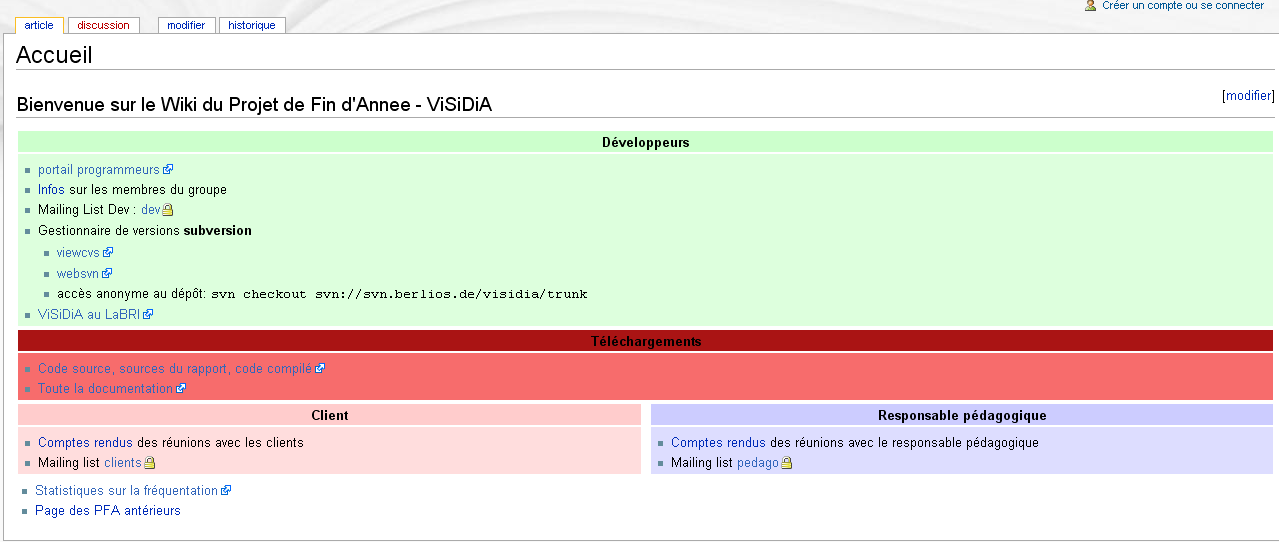
\includegraphics[width=16cm]{images/wiki.png}
  \caption{Le wiki du projet Visidia}
\end{figure}

Nous avons d�ploy�s plusieurs listes de diffusion pour faciliter la communication :
\begin{itemize}
  \item Une liste pour tous les d�veloppeurs
  \item Une liste de diffusion pour communiquer avec le client
  \item Une liste de diffusion pour communiquer avec le responsable p�dagogique \\
\end{itemize}

Nous avons utilis� �galement un gestionnaire de versions, Subversion
, qui nous permet de maintenir les sources de \visidia. 
Les clients ont �galement la possibilit� de
suivre l'avancement du projet et d'acc�der aux sources, gr�ce � deux
interfaces viewcvs  et websvn .  Il est
�galement possible de t�l�charger la derni�re version des sources du
projet:
\begin{verbatim}
svn checkout svn://svn.berlios.de/visidia/trunk
\end{verbatim}


\section{Organisation du travail}

Notre groupe de travail �tant form� de 6 personnes, nous avons d�cid�s de former
trois bin�mes afin de favoriser et optimiser le travail en �quipe. 
De plus la formation de binome permettait de mettre en place le systeme
d�veloppeur/relecteur, et facilite l'appr�hension d'une application comme
\visidia, puisque chacun pouvait expliquer � son partenaire les concepts qu'il avait
saisi pour mututellement enrichir ses connaissances de l'application.\\

Nous nous sommes r�parti le travail de mani�re � faire en sorte, que les binomes
form�s n'ait � se concentrer essentiellement que sur une partie du d�veloppement
de \visidia. Ainsi nous avons eu un binom� charg� d'impl�menter les
fonctionnalit�s relatives aux graphes et un autre celles relatives aux agents.

\section{Avancement du projet}

\begin{figure}[!ht]
  \center
  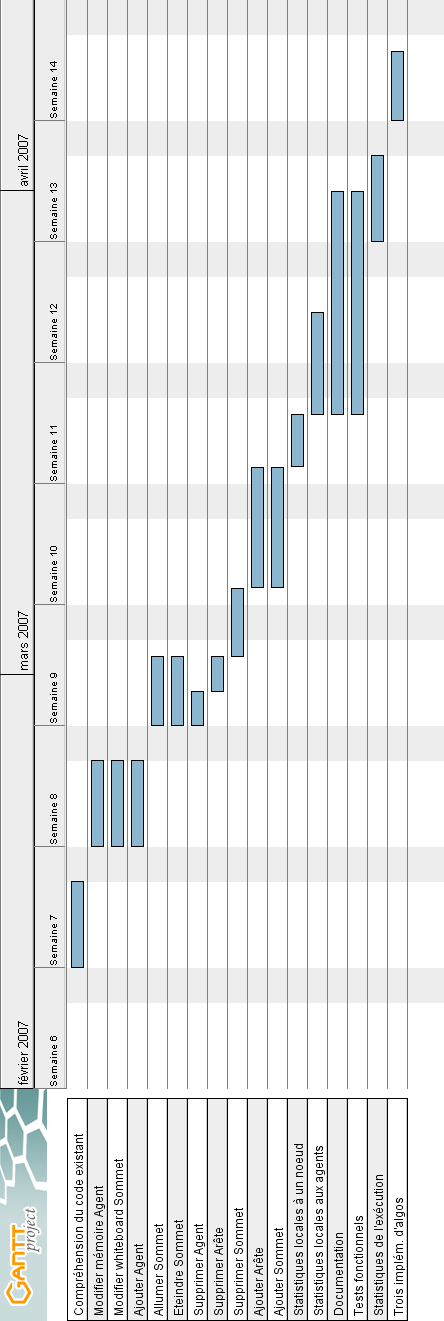
\includegraphics[height=20cm]{images/gantt2.png}
  \caption{Diagramme de Gantt}
\end{figure}
%diagramme de gant a mettre la


